\documentclass[11pt,a4paper]{article}

% ==================== PACKAGES ====================
\usepackage[a4paper, margin=1in]{geometry}
\usepackage{amsmath,amssymb,amsthm,mathtools}
\usepackage{graphicx}
\usepackage{float}
\usepackage{booktabs}
\usepackage{array}
\usepackage{multirow}
\usepackage{longtable}
\usepackage{tabularx}
\usepackage{caption}
\usepackage{subcaption}
\usepackage[table]{xcolor}
\usepackage{colortbl}
\usepackage{tikz}
\usepackage{pgfplots}
\usepackage{enumitem}
\usepackage[protrusion=true,expansion=false]{microtype}
\usepackage{textcomp}
\usepackage[T1]{fontenc}
\usepackage[utf8]{inputenc}
\usepackage[hidelinks,colorlinks=true,linkcolor=teal!70!black,citecolor=blue!60!black,urlcolor=teal!70!black]{hyperref}
\usepackage[noabbrev]{cleveref}
\usepackage{lipsum}

\usetikzlibrary{positioning,arrows.meta,shapes,calc,decorations.pathreplacing,patterns}
\pgfplotsset{compat=1.18}

% Custom colours
\definecolor{titleblue}{RGB}{30,60,114}
\definecolor{accent}{RGB}{198,40,40}
\definecolor{accentgreen}{RGB}{46,125,50}
\definecolor{lightbg}{RGB}{245,247,250}
\definecolor{tablerow}{RGB}{232,238,247}

% Caption styling
\captionsetup[figure]{labelfont={bf,color=titleblue},textfont=small,skip=4pt}
\captionsetup[table]{labelfont={bf,color=titleblue},textfont=small,skip=4pt,position=above}

% Section style
\usepackage{titlesec}
\titleformat{\section}{\Large\bfseries\color{titleblue}}{\thesection}{0.6em}{}
\titleformat{\subsection}{\large\bfseries\color{titleblue!85!black}}{\thesubsection}{0.5em}{}
\titleformat{\subsubsection}{\normalsize\bfseries\color{titleblue!70!black}}{\thesubsubsection}{0.4em}{}

% Maths shortcuts
\newcommand{\vff}{v_{\mathrm{ff}}}
\newcommand{\Tff}{T_{\mathrm{ff}}}
\newcommand{\veh}{\mathrm{veh}}

% Data macros
% Auto-generated data macros from SUMO 12 scenarios
\newcommand{\dPBaseCap}{6457.6}
\newcommand{\dPBaseThr}{4582.9}
\newcommand{\dPBaseDelay}{11.89}
\newcommand{\dPBasePkDelay}{23.45}
\newcommand{\dPBaseQueue}{17.24}
\newcommand{\dPBasePkQueue}{29.77}
\newcommand{\dPBaseTimeQ}{0.46}
\newcommand{\dPBaseExcAcc}{17.24}
\newcommand{\dPBasePkExcAcc}{29.77}
\newcommand{\dPBaseTimeLoss}{143396.6}
\newcommand{\dPBaseSpeed}{48.96}
\newcommand{\dPBaseNetDelay}{31.92}
\newcommand{\dPVslCap}{6286.7}
\newcommand{\dPVslThr}{4091.1}
\newcommand{\dPVslDelay}{13.17}
\newcommand{\dPVslPkDelay}{24.58}
\newcommand{\dPVslQueue}{17.03}
\newcommand{\dPVslPkQueue}{29.97}
\newcommand{\dPVslTimeQ}{0.481}
\newcommand{\dPVslExcAcc}{17.03}
\newcommand{\dPVslPkExcAcc}{29.97}
\newcommand{\dPVslTimeLoss}{173427.1}
\newcommand{\dPVslSpeed}{47.08}
\newcommand{\dPVslNetDelay}{38.6}
\newcommand{\dPVslUpCap}{7388.4}
\newcommand{\dPVslUpThr}{4661.7}
\newcommand{\dPVslUpDelay}{11.49}
\newcommand{\dPVslUpPkDelay}{18.48}
\newcommand{\dPVslUpQueue}{16.87}
\newcommand{\dPVslUpPkQueue}{26.13}
\newcommand{\dPVslUpTimeQ}{0.207}
\newcommand{\dPVslUpExcAcc}{16.87}
\newcommand{\dPVslUpPkExcAcc}{26.13}
\newcommand{\dPVslUpTimeLoss}{142331.4}
\newcommand{\dPVslUpSpeed}{49.41}
\newcommand{\dPVslUpNetDelay}{31.68}
\newcommand{\dPRmCap}{7209.3}
\newcommand{\dPRmThr}{4736.5}
\newcommand{\dPRmDelay}{10.97}
\newcommand{\dPRmPkDelay}{23.19}
\newcommand{\dPRmQueue}{15.7}
\newcommand{\dPRmPkQueue}{26.18}
\newcommand{\dPRmTimeQ}{0.22}
\newcommand{\dPRmExcAcc}{15.7}
\newcommand{\dPRmPkExcAcc}{26.18}
\newcommand{\dPRmTimeLoss}{110833.5}
\newcommand{\dPRmSpeed}{50.84}
\newcommand{\dPRmNetDelay}{24.67}
\newcommand{\dPVslRmCap}{6390.8}
\newcommand{\dPVslRmThr}{4219.8}
\newcommand{\dPVslRmDelay}{13.8}
\newcommand{\dPVslRmPkDelay}{24.34}
\newcommand{\dPVslRmQueue}{17.23}
\newcommand{\dPVslRmPkQueue}{26.98}
\newcommand{\dPVslRmTimeQ}{0.531}
\newcommand{\dPVslRmExcAcc}{17.23}
\newcommand{\dPVslRmPkExcAcc}{26.98}
\newcommand{\dPVslRmTimeLoss}{173335.5}
\newcommand{\dPVslRmSpeed}{45.77}
\newcommand{\dPVslRmNetDelay}{38.58}
\newcommand{\dPVslUpRmCap}{7253.4}
\newcommand{\dPVslUpRmThr}{4582.3}
\newcommand{\dPVslUpRmDelay}{11.03}
\newcommand{\dPVslUpRmPkDelay}{21.51}
\newcommand{\dPVslUpRmQueue}{15.46}
\newcommand{\dPVslUpRmPkQueue}{25.63}
\newcommand{\dPVslUpRmTimeQ}{0.246}
\newcommand{\dPVslUpRmExcAcc}{15.46}
\newcommand{\dPVslUpRmPkExcAcc}{25.63}
\newcommand{\dPVslUpRmTimeLoss}{123997.1}
\newcommand{\dPVslUpRmSpeed}{50.75}
\newcommand{\dPVslUpRmNetDelay}{27.6}
\newcommand{\dOBaseCap}{6752.6}
\newcommand{\dOBaseThr}{5171.2}
\newcommand{\dOBaseDelay}{9.31}
\newcommand{\dOBasePkDelay}{15.43}
\newcommand{\dOBaseQueue}{15.14}
\newcommand{\dOBasePkQueue}{24.16}
\newcommand{\dOBaseTimeQ}{0.078}
\newcommand{\dOBaseExcAcc}{15.14}
\newcommand{\dOBasePkExcAcc}{24.16}
\newcommand{\dOBaseTimeLoss}{89050.3}
\newcommand{\dOBaseSpeed}{53.53}
\newcommand{\dOBaseNetDelay}{16.2}
\newcommand{\dOVslCap}{6471.4}
\newcommand{\dOVslThr}{4658.4}
\newcommand{\dOVslDelay}{12.52}
\newcommand{\dOVslPkDelay}{19.94}
\newcommand{\dOVslQueue}{18.26}
\newcommand{\dOVslPkQueue}{29.95}
\newcommand{\dOVslTimeQ}{0.301}
\newcommand{\dOVslExcAcc}{18.26}
\newcommand{\dOVslPkExcAcc}{29.95}
\newcommand{\dOVslTimeLoss}{167590.0}
\newcommand{\dOVslSpeed}{47.7}
\newcommand{\dOVslNetDelay}{30.49}
\newcommand{\dOVslUpCap}{6862.2}
\newcommand{\dOVslUpThr}{5178.6}
\newcommand{\dOVslUpDelay}{9.78}
\newcommand{\dOVslUpPkDelay}{16.38}
\newcommand{\dOVslUpQueue}{15.8}
\newcommand{\dOVslUpPkQueue}{25.78}
\newcommand{\dOVslUpTimeQ}{0.046}
\newcommand{\dOVslUpExcAcc}{15.8}
\newcommand{\dOVslUpPkExcAcc}{25.78}
\newcommand{\dOVslUpTimeLoss}{99602.3}
\newcommand{\dOVslUpSpeed}{52.49}
\newcommand{\dOVslUpNetDelay}{18.12}
\newcommand{\dORmCap}{7402.0}
\newcommand{\dORmThr}{4926.0}
\newcommand{\dORmDelay}{8.65}
\newcommand{\dORmPkDelay}{13.05}
\newcommand{\dORmQueue}{13.54}
\newcommand{\dORmPkQueue}{24.43}
\newcommand{\dORmTimeQ}{0.053}
\newcommand{\dORmExcAcc}{13.54}
\newcommand{\dORmPkExcAcc}{24.43}
\newcommand{\dORmTimeLoss}{86585.3}
\newcommand{\dORmSpeed}{55.12}
\newcommand{\dORmNetDelay}{15.75}
\newcommand{\dOVslRmCap}{6392.6}
\newcommand{\dOVslRmThr}{4409.8}
\newcommand{\dOVslRmDelay}{10.7}
\newcommand{\dOVslRmPkDelay}{31.06}
\newcommand{\dOVslRmQueue}{14.88}
\newcommand{\dOVslRmPkQueue}{24.07}
\newcommand{\dOVslRmTimeQ}{0.179}
\newcommand{\dOVslRmExcAcc}{14.88}
\newcommand{\dOVslRmPkExcAcc}{24.07}
\newcommand{\dOVslRmTimeLoss}{140242.1}
\newcommand{\dOVslRmSpeed}{51.41}
\newcommand{\dOVslRmNetDelay}{25.52}
\newcommand{\dOVslUpRmCap}{6701.5}
\newcommand{\dOVslUpRmThr}{4652.7}
\newcommand{\dOVslUpRmDelay}{9.13}
\newcommand{\dOVslUpRmPkDelay}{19.12}
\newcommand{\dOVslUpRmQueue}{13.62}
\newcommand{\dOVslUpRmPkQueue}{24.76}
\newcommand{\dOVslUpRmTimeQ}{0.062}
\newcommand{\dOVslUpRmExcAcc}{13.62}
\newcommand{\dOVslUpRmPkExcAcc}{24.76}
\newcommand{\dOVslUpRmTimeLoss}{107329.5}
\newcommand{\dOVslUpRmSpeed}{54.19}
\newcommand{\dOVslUpRmNetDelay}{19.53}


% ==================== METADATA ====================
\title{\vspace{-2em}\textbf{Analysis and Mitigation of the AYE Westbound Weaving Bottleneck}\\[0.4em]
\large CE5203 Traffic Flow and Control --- Course Project, Spring 2026\\[0.6em]
\rule{0.7\textwidth}{0.6pt}}

\author{
\textbf{Group 12} \\[0.2em]
Leong Sio Kuan \quad Luo Wenjie \\[0.2em]
Wang Xu \quad Zhao Jiaqing \\[0.2em]
\small Department of Civil and Environmental Engineering, National University of Singapore
}
\date{26 April 2026}

\begin{document}
\maketitle

% ==================== ABSTRACT ====================
\begin{abstract}
\noindent
We study a recurring bottleneck on Singapore's Ayer Rajah Expressway (AYE) westbound between Exit 9 (Clementi-bound on-ramp) and Exit 11 (Clementi off-ramp). A 46-min peak-period and 62-min off-peak field survey was conducted; vehicles were counted by class with a YOLOv11 pipeline at four measurement points. The empirical capacity of the 373\,m weaving section is approximately \textbf{5{,}060\,veh/h}, with peak-period total upstream flow of 5{,}060\,veh/h (51.2\,\% car exit ratio, 1{,}785\,veh/h ramp-merge flow) and off-peak flow of 5{,}050\,veh/h (40.6\,\% exit ratio, 1{,}185\,veh/h ramp-merge). A SUMO microsimulation calibrated to the YOLO speed/demand data was used to compute the four traffic performance parameters required by the project brief and to evaluate three control strategies --- Variable Speed Limit (VSL), Ramp Metering (RM), and a combined VSL$+$RM --- across both peak and off-peak demand profiles, plus a literature-recommended upstream VSL placement, giving \textbf{12 simulation runs}. Ramp metering at a 20\,\% downstream-occupancy threshold is the only consistently beneficial strategy: peak-period network total time loss decreased by \textbf{22.7\,\%} and average delay on the weaving section by \textbf{7.7\,\%}, with negligible effect during off-peak. In-section VSL on a single weaving lane degraded performance in both periods; relocating VSL upstream to the mainline removed most of the harm but did not match RM. We recommend deploying ramp metering alone on this site.
\end{abstract}

\vspace{0.5em}\noindent\textit{Keywords:} weaving bottleneck, ramp metering, variable speed limit, microsimulation, SUMO, ALINEA, AYE Singapore.

\tableofcontents
\newpage

% ==================== SECTION 1 ====================
\section{Introduction}
\label{sec:intro}
The Ayer Rajah Expressway (AYE) connects Singapore's central business district to the western residential and industrial districts \cite{onemotoring,bib:aye}. During evening peaks, severe congestion is observed on the westbound carriageway between Exit 9 and Exit 11, where a 1\,lane on-ramp from Clementi/Buona Vista feeds traffic into the mainline immediately upstream of the Exit 11 (Clementi) off-ramp. The two opposing lane-change movements --- merging vehicles from lane~0 and exiting vehicles from lanes 2 and 3 of the upstream mainline --- compete within a $373$\,m weaving section, producing speed drops, queue spillback and elevated travel times.

\paragraph{Project task.}
Following the CE5203 brief, this project: (a) identifies the source of congestion; (b) computes the capacity of the system during the peak period; (c) computes at least two of the four required parameters (we report all four: average delay, average queue length, average time in queue, average excess accumulation); (d) repeats (b) and (c) for the off-peak period; (e) proposes and evaluates a control strategy in both periods.

\paragraph{Approach.}
The bottleneck location was first identified from LTA OneMotoring traffic-condition data and a field survey from College Link Road. A digital camera at a footbridge and a smartphone facing the exit recorded 46 minutes of peak traffic on 19~March 2026 and 62 minutes of off-peak traffic on 24~March 2026. A YOLOv11 vehicle-counting pipeline extracted per-minute flows by class. A SUMO microsimulation of the weaving section, calibrated to the YOLO data, was then used to compute the four performance parameters and to evaluate three control strategies (VSL, ramp metering, VSL$+$RM) plus an upstream-VSL alternative.

\Cref{fig:network} shows the network layout reproduced in SUMO. The weaving section between the merge node and the diverge node contains four physical lanes (the additional left-most lane originates from the on-ramp); the upstream mainline (E\_main\_in) and downstream mainline (E\_main\_out) carry three lanes each.

\begin{figure}[H]
\centering
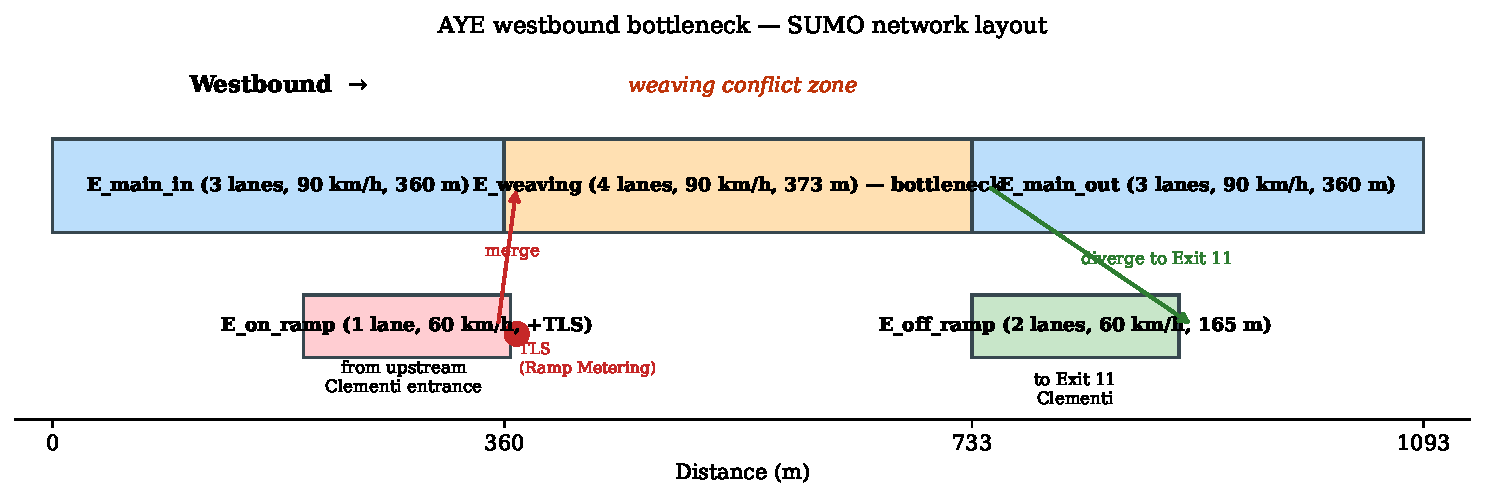
\includegraphics[width=0.98\linewidth]{figs/fig_network.pdf}
\caption{AYE westbound bottleneck reproduced as a SUMO network. The 373\,m weaving section between merge and diverge nodes is the primary bottleneck. Length, lane count and speed limit per edge are shown.}
\label{fig:network}
\end{figure}

% ==================== SECTION 2 ====================
\section{Field Survey and YOLO Vehicle Counting}
\label{sec:survey}

\subsection{Field Survey}
The peak survey ran from 18:31--19:14 on 19~March 2026 (3 minutes of low-quality data discarded, 43 valid minutes); the off-peak survey ran from 14:05--15:07 on 24~March 2026 (2 minutes discarded, 60 valid minutes). The mainline speed limit is 90\,km/h (60\,km/h for buses/coaches/large trucks); ramp speed limit is 50\,km/h. Heavy vehicle composition was small in both periods.

\subsection{YOLO Vehicle Counting}
\label{sec:yolo}
We use the YOLOv11 pre-trained model (chosen over the latest YOLOv26 for compatibility with the laptop GPU) to detect cars, motorcycles, buses and trucks frame by frame. Virtual detection lines on the video acted as loop detectors. To reduce double-counting we grouped overlapping detection lines so that a vehicle could only register once per group. Counts at the merge and exit measurement points were corrected using the formulas
\begin{align}
\text{Exit volume} &= V_{\text{exit lane (line)}} + V_{\text{LC-left after line}}, \label{eq:yolo1} \\
\text{Mainline after exit} &= V_{\text{mainline (line)}} - V_{\text{LC-left after line}}, \label{eq:yolo2}
\end{align}
where $V_{\text{LC-left after line}}$ is the count of vehicles that performed a leftward lane change downstream of the detection line. The processed counts are summarised in \cref{tab:survey}; the per-minute demand profile generated from the YOLO data is shown in \cref{fig:demand}.

\begin{table}[H]
\centering
\caption{Field survey summary (excluding motorcycles).}
\label{tab:survey}
\rowcolors{2}{tablerow}{white}
\begin{tabular}{lrrrr}
\toprule
\textbf{Parameter} & \textbf{Peak} & \textbf{Off-Peak} & \textbf{$\Delta$} & \textbf{Unit} \\ \midrule
Survey duration            & 43    & 60    & --     & min \\
Total upstream flow        & 3{,}627 & 5{,}050 & --   & veh \\
Flow rate                  & 5{,}060 & 5{,}050 & $-0.2\%$ & veh/h \\
Mainline flow              & 3{,}276 & 3{,}865 & $+18\%$  & veh/h \\
On-ramp merge flow         & 1{,}785 & 1{,}185 & $-34\%$  & veh/h \\
Exit flow                  & 2{,}393 & 1{,}774 & $-26\%$  & veh/h \\
Exit ratio (cars)          & 51.2\,\% & 40.6\,\% & --   & -- \\
\bottomrule
\end{tabular}
\end{table}

\begin{figure}[H]
\centering
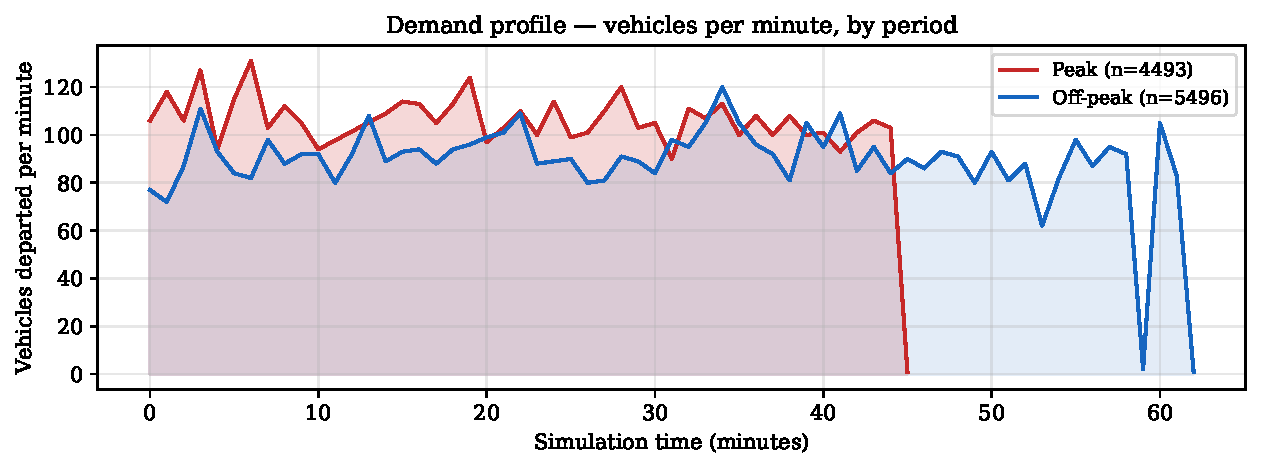
\includegraphics[width=0.95\linewidth]{figs/fig_demand.pdf}
\caption{Demand profile per minute, derived from YOLO counts. Peak demand spans 0--45\,min with a maximum of about 110\,veh/min; off-peak demand spans 0--62\,min with a more uniform profile.}
\label{fig:demand}
\end{figure}

% ==================== SECTION 3 ====================
\section{Analysis During the Peak Period}
\label{sec:peak}

\subsection{Source of Congestion}
\label{sec:source}
The primary bottleneck is the 373\,m weaving section between the on-ramp merge node and the off-ramp diverge node. Three conflicting movements coexist on it:
\begin{enumerate}[topsep=2pt,itemsep=1pt]
\item merging vehicles entering at lane~0 must change lanes rightward to join through-traffic;
\item exit-bound vehicles need to change lanes leftward to reach lane~0 or lane~1;
\item through-traffic competes for the remaining lanes.
\end{enumerate}
During the peak survey, $51.2\%$ of cars exited and the upstream on-ramp merged a flow of $1{,}785$\,veh/h --- a $50\%$ increase over off-peak. The combined lane-change demand exceeds the section's ability to accommodate smooth weaving and queue spillback propagates upstream.

\subsection{Capacity Estimation}
\label{sec:capacity}
Capacity was estimated from the YOLO upstream count over the peak survey:
\begin{equation}
\hat{C}_{\text{peak}} \;=\; \frac{N_{\text{upstream}}}{T_{\text{survey}}}\;=\;\frac{3{,}627\,\veh}{43/60\,\mathrm{h}}\;\approx\;5{,}060\,\veh/\mathrm{h}.
\label{eq:capacity}
\end{equation}
The downstream measurement gave $5{,}231$\,veh/h, which agrees with \cref{eq:capacity} to within typical YOLO counting error. Off-peak total upstream flow was $5{,}050$\,veh/h over $60$\,min, essentially identical, indicating that the section operates near its empirical capacity in both periods (\cref{tab:survey}).

\subsection{SUMO Microsimulation Setup}
\label{sec:sumo}
A SUMO model of the network in \cref{fig:network} was built with seven nodes, six edges and nine lane-level connections (\cref{tab:edges,tab:connections}). The SUMO Krauss car-following model was used (default in SUMO), and the SL2015 sublane lane-changing model was activated by setting \texttt{lateral-resolution = 0.8\,m}, dividing each $3.2$\,m lane into four lateral strips.

\begin{table}[H]
\centering
\caption{Edge topology.}
\label{tab:edges}
\rowcolors{2}{tablerow}{white}
\begin{tabular}{l c c c c l}
\toprule
\textbf{Edge ID} & \textbf{Lanes} & \textbf{Length (m)} & \textbf{Speed (m/s)} & \textbf{[km/h]} & \textbf{Function} \\ \midrule
E\_main\_in    & 3 & 360 & 25.00 & [90] & Upstream mainline \\
E\_on\_ramp\_1 & 1 & 103 & 16.67 & [60] & On-ramp before TLS \\
E\_on\_ramp\_2 & 1 & 62  & 16.67 & [60] & On-ramp after TLS \\
E\_weaving     & 4 & 373 & 25.00 & [90] & Weaving (bottleneck) \\
E\_main\_out   & 3 & 360 & 25.00 & [90] & Downstream mainline \\
E\_off\_ramp   & 2 & 165 & 16.67 & [60] & Exit ramp (Exit 11) \\
\bottomrule
\end{tabular}
\end{table}

\begin{table}[H]
\centering
\caption{Lane connections of the weaving conflict.}
\label{tab:connections}
\rowcolors{2}{tablerow}{white}
\begin{tabular}{lc c lc}
\toprule
\textbf{From edge} & \textbf{From lane} & \textbf{$\rightarrow$} & \textbf{To edge} & \textbf{To lane} \\ \midrule
E\_main\_in   & 0 & $\rightarrow$ & E\_weaving   & 1 \\
E\_main\_in   & 1 & $\rightarrow$ & E\_weaving   & 2 \\
E\_main\_in   & 2 & $\rightarrow$ & E\_weaving   & 3 \\
E\_on\_ramp\_2& 0 & $\rightarrow$ & E\_weaving   & 0 \\
E\_weaving    & 0 & $\rightarrow$ & E\_off\_ramp & 0 \\
E\_weaving    & 1 & $\rightarrow$ & E\_off\_ramp & 1 \\
E\_weaving    & 1 & $\rightarrow$ & E\_main\_out & 0 \\
E\_weaving    & 2 & $\rightarrow$ & E\_main\_out & 1 \\
E\_weaving    & 3 & $\rightarrow$ & E\_main\_out & 2 \\
\bottomrule
\end{tabular}
\end{table}

\subsubsection{Krauss car-following model}
The follower's safe speed satisfies the Gipps safe-distance condition,
\begin{equation}
v_{\text{safe}} \;=\; v_{\text{lead}} + \frac{g - v_{\text{lead}}\,\tau}{\dfrac{v_{\text{follow}}+v_{\text{lead}}}{2b} + \tau},
\label{eq:vsafe}
\end{equation}
where $g$ is the bumper-to-bumper gap, $\tau$ the desired headway/reaction time and $b$ the comfortable deceleration. The realised speed is
\begin{equation}
v_{\text{next}} \;=\; \max\!\left[0,\;\min(v_{\text{des}}, v_{\text{safe}}, v_{\text{cur}}+a\Delta t) - \sigma\,\xi\,a\,\Delta t\right],
\label{eq:vnext}
\end{equation}
with stochastic imperfection $\sigma\in[0,1]$, $\xi\sim U(0,1)$, simulation step $\Delta t$, maximum acceleration $a$, and individual desired speed
\begin{equation}
v_{\text{des}} \;=\; v_{\text{limit}}\cdot\mathcal{N}(\mu_{\text{spd}},\sigma_{\text{spd}}).
\label{eq:vdes}
\end{equation}
Calibration values per vehicle class are given in \cref{tab:krauss}.

\begin{table}[H]
\centering
\caption{Krauss car-following parameters (speeds in m/s; km/h equivalents in brackets where useful).}
\label{tab:krauss}
\rowcolors{2}{tablerow}{white}
\begin{tabular}{lcccc}
\toprule
\textbf{Parameter} & \textbf{Car} & \textbf{Motorcycle} & \textbf{Bus} & \textbf{Truck} \\ \midrule
length (m)         & 4.5 & 2.2 & 12.0 & 8.0 \\
minGap (m)         & 1.5 & 1.0 & 2.5  & 2.0 \\
maxSpeed (m/s) [km/h] & 27.0 [97] & 25.0 [90] & 25.0 [90] & 28.0 [101] \\
$a$ (m/s$^2$)      & 2.6 & 3.5 & 1.2 & 1.0 \\
$b$ (m/s$^2$)      & 4.5 & 5.0 & 4.0 & 3.5 \\
$\sigma$           & 0.5 & 0.5 & 0.4 & 0.4 \\
$\tau$ (s)         & 0.8 & 0.6 & 1.0 & 1.0 \\
$\mu_{\text{spd}}$ & 0.84 & 0.80 & 0.72 & 0.76 \\
$\sigma_{\text{spd}}$ & 0.10 & 0.12 & 0.10 & 0.08 \\
\bottomrule
\end{tabular}
\end{table}

\subsubsection{SL2015 sublane lane-changing model}
Lane-change desirability is the sum of strategic, cooperative, speed-gain and keep-right utilities:
\begin{equation}
U \;=\; U_{\text{strategic}} + U_{\text{cooperative}} + U_{\text{speedGain}} + U_{\text{keepRight}},
\label{eq:lcutil}
\end{equation}
with
\begin{equation}
U_{\text{strategic}} \propto \frac{\text{lcStrategic}}{d_{\text{remaining}}},\qquad
g_{\text{required}} \;=\; \frac{g_{\text{safe}}}{\text{lcAssertive}}.
\label{eq:lcassert}
\end{equation}
We use $\text{lcStrategic}_{\text{car}}=10$, $\text{lcAssertive}_{\text{car}}=2$ (motorcycle 3.0, due to narrow width), and $\text{lcKeepRight}=0$ for all classes (Singapore expressways do not enforce slow-lane return under congestion).

\subsubsection{Demand and speed calibration}
\label{sec:demand}
Demand was generated from per-minute YOLO counts; departure times were sampled uniformly within each 60\,s interval. \Cref{tab:routes} lists the four routes and their vehicle counts.

\begin{table}[H]
\centering
\caption{Routes and vehicle counts driving the SUMO simulation.}
\label{tab:routes}
\rowcolors{2}{tablerow}{white}
\begin{tabular}{l l c c}
\toprule
\textbf{Route} & \textbf{Edges} & \textbf{Peak} & \textbf{Off-Peak} \\ \midrule
route\_main\_through & E\_main\_in $\to$ E\_weaving $\to$ E\_main\_out & 1{,}796 & 2{,}751 \\
route\_main\_to\_exit & E\_main\_in $\to$ E\_weaving $\to$ E\_off\_ramp & 1{,}343 & 1{,}475 \\
route\_ramp\_merge & E\_on\_ramp $\to$ E\_weaving $\to$ E\_main\_out & 1{,}225 & 1{,}159 \\
route\_ramp\_to\_exit & E\_on\_ramp $\to$ E\_weaving $\to$ E\_off\_ramp & 129 & 111 \\ \midrule
\textbf{Total} & --- & \textbf{4{,}493} & \textbf{5{,}496} \\ \bottomrule
\end{tabular}
\end{table}

The desired-speed factor $\mu_{\text{spd}}$ was calibrated from off-peak Group~1 (fastest-lane) speed sampling in the YOLO data, which best approximates free-flow conditions. Identical values were used in both peak and off-peak runs so that performance differences come from demand alone.

\subsubsection{Simulation configuration}
$\Delta t = 0.5$\,s, simulation duration $5{,}400$\,s, fixed seed $42$. Per-edge metrics are written every 60\,s through SUMO's \texttt{edgeData} collector. The simulations were driven by the libsumo Python binding.

\subsection{Peak Period Performance Parameters}
\label{sec:peakperf}
The four parameters required by the brief are computed from the SUMO base-peak run (\cref{tab:peakperf}). \Cref{fig:funddiag} (a) plots the resulting density-flow scatter for each edge --- the weaving edge sits clearly in the congested branch, while upstream and downstream mainline points cluster in the free-flow branch. Per-edge speed comparison (\cref{fig:peredge}) confirms the weaving edge is the hot spot.

\subsubsection{Average delay}
\begin{equation}
\Tff \;=\; \frac{L_{\mathrm{w}}}{\vff} \;=\; \frac{373.01\,\mathrm{m}}{25.0\,\mathrm{m/s}} \;\approx\; 14.92\,\mathrm{s}.
\label{eq:tff}
\end{equation}
\begin{equation}
\bar{d} \;=\; \mathbb{E}\!\left[T_{\text{travel}}\right] - \Tff \;=\; \dPBaseDelay\,\mathrm{s/veh}.
\label{eq:delay}
\end{equation}

\subsubsection{Average queue length}
\begin{equation}
Q \;=\; k\cdot L_{\mathrm{w}}\cdot \left(1 - \frac{v}{\vff}\right),
\label{eq:queue}
\end{equation}
where $k$ is density (veh/km) and the factor $(1-v/\vff)$ isolates the congested fraction. Average $Q = \dPBaseQueue$\,veh; peak $Q = \dPBasePkQueue$\,veh ($\approx \dPBasePkQueue\times 5.6 / 100 \approx 167$\,m).

\subsubsection{Average time in queue}
The average time spent at near-zero speed (below $0.1$\,m/s) on the weaving section was $\dPBaseTimeQ$\,s/veh.

\subsubsection{Average excess accumulation (Little's Law)}
With arrival rate $\lambda$,
\begin{equation}
N_{\text{opt}} \;=\; \lambda\,\Tff,\qquad N_{\text{excess}} \;=\; N_{\text{actual}} - N_{\text{opt}}.
\label{eq:excess}
\end{equation}
Average $N_{\text{excess}} = \dPBaseExcAcc$\,veh; peak $\dPBasePkExcAcc$\,veh.

\begin{table}[H]
\centering
\caption{Peak-period performance parameters on the weaving section (E\_weaving), from base SUMO run.}
\label{tab:peakperf}
\rowcolors{2}{tablerow}{white}
\begin{tabular}{l r r l}
\toprule
\textbf{Parameter} & \textbf{Average} & \textbf{Peak interval} & \textbf{Unit} \\ \midrule
Average delay         & \dPBaseDelay  & \dPBasePkDelay  & s/veh \\
Average queue length  & \dPBaseQueue  & \dPBasePkQueue  & vehicles \\
Time in queue         & \dPBaseTimeQ  & ---             & s/veh \\
Excess accumulation   & \dPBaseExcAcc & \dPBasePkExcAcc & vehicles \\
Net total time loss (network) & \dPBaseTimeLoss & --- & veh-s \\
Avg weaving speed     & \dPBaseSpeed  & ---             & km/h \\
Capacity (instantaneous) & \dPBaseCap & ---             & veh/h \\
\bottomrule
\end{tabular}
\end{table}

\begin{figure}[H]
\centering
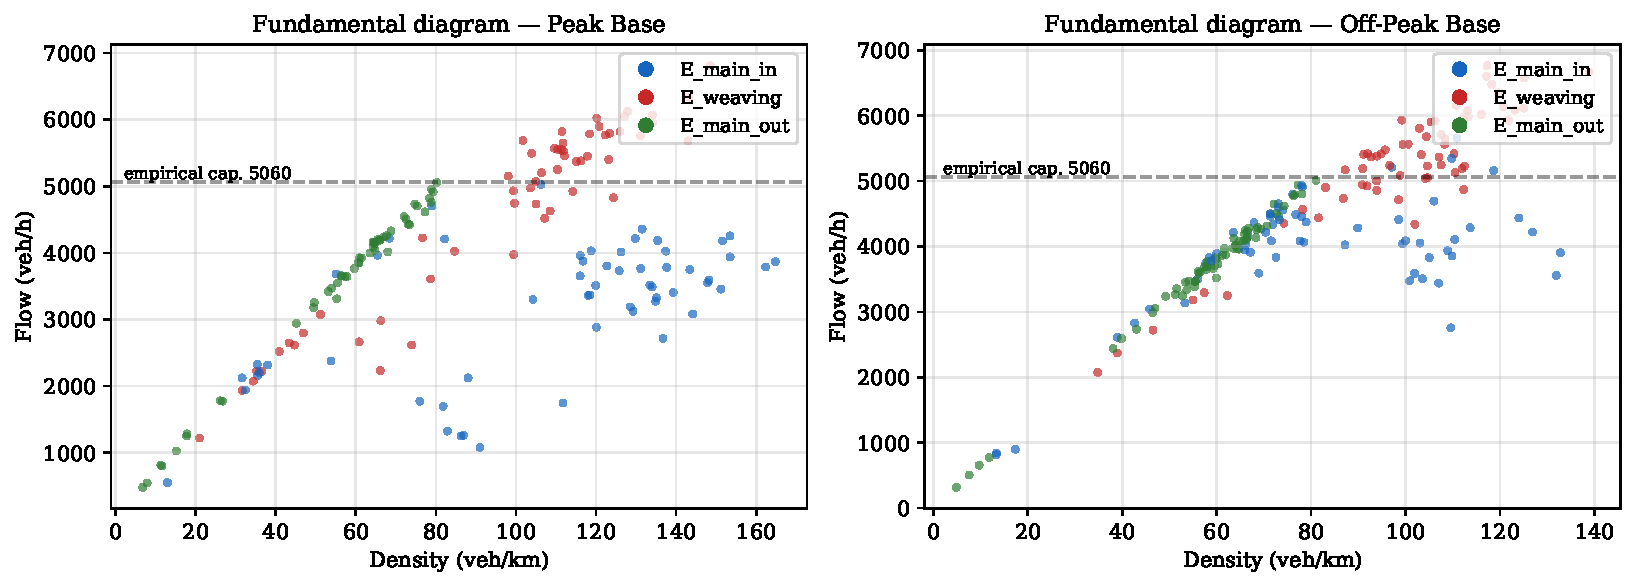
\includegraphics[width=0.95\linewidth]{figs/fig_funddiag.pdf}
\caption{Empirical fundamental diagram per edge, peak vs off-peak. Red points (E\_weaving) lie in the congested branch during peak; blue and green points stay in the free-flow branch. The dashed line marks the empirical capacity from \cref{eq:capacity}.}
\label{fig:funddiag}
\end{figure}

\begin{figure}[H]
\centering
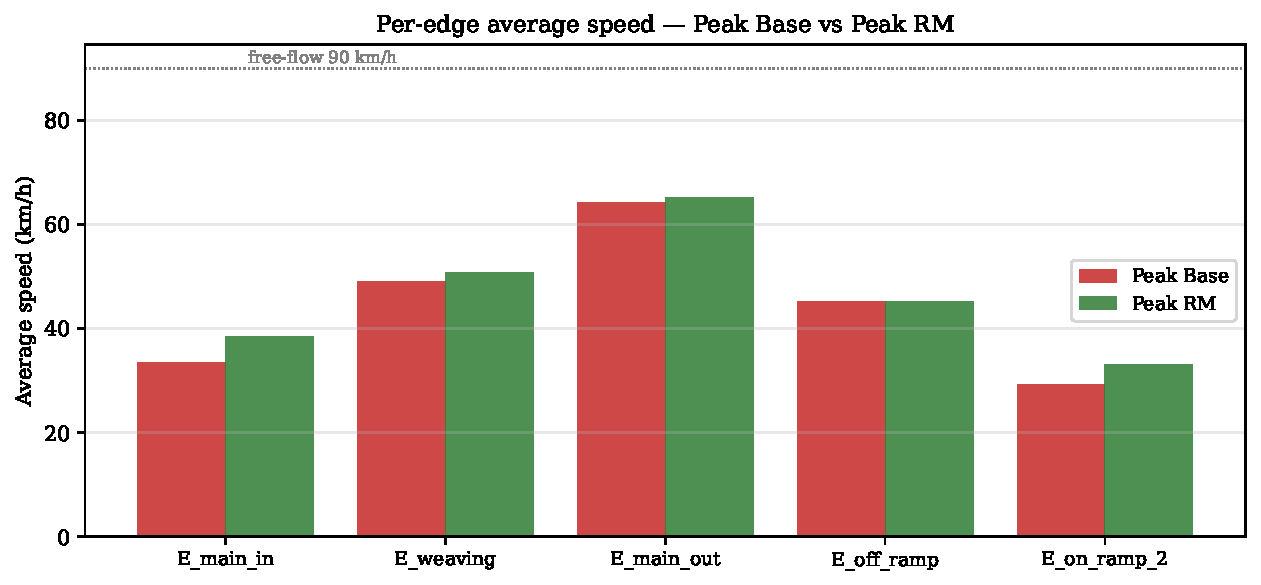
\includegraphics[width=0.85\linewidth]{figs/fig_per_edge_speed.pdf}
\caption{Per-edge average speed --- the weaving edge is the slowest in both base and RM scenarios. RM brings the weaving speed up by about $4$\,km/h while leaving the upstream mainline largely unaffected.}
\label{fig:peredge}
\end{figure}

% ==================== SECTION 4 ====================
\section{Analysis During the Off-Peak Period}
\label{sec:off}

\subsection{Conditions and capacity}
The off-peak total upstream flow was $5{,}050$\,veh/h over $60$\,min, almost identical in magnitude to the peak. The differences are in composition: mainline flow $3{,}865$\,veh/h (up from $3{,}276$ peak), exit flow $1{,}774$\,veh/h (down from $2{,}393$), on-ramp flow $1{,}185$\,veh/h (down from $1{,}785$); car exit ratio dropped from 51.2\,\% to 40.6\,\%. Off-peak car speeds averaged $61$\,km/h on the mainline, against $45$\,km/h during peak.

\subsection{Off-peak performance parameters}
The same four parameters are reported in \cref{tab:offperf}, drawn from the SUMO base-offpeak simulation.

\begin{table}[H]
\centering
\caption{Off-peak performance parameters (E\_weaving, base SUMO).}
\label{tab:offperf}
\rowcolors{2}{tablerow}{white}
\begin{tabular}{l r r l}
\toprule
\textbf{Parameter} & \textbf{Average} & \textbf{Peak interval} & \textbf{Unit} \\ \midrule
Average delay         & \dOBaseDelay  & \dOBasePkDelay  & s/veh \\
Average queue length  & \dOBaseQueue  & \dOBasePkQueue  & vehicles \\
Time in queue         & \dOBaseTimeQ  & ---             & s/veh \\
Excess accumulation   & \dOBaseExcAcc & \dOBasePkExcAcc & vehicles \\
Net total time loss (network) & \dOBaseTimeLoss & --- & veh-s \\
Avg weaving speed     & \dOBaseSpeed  & ---             & km/h \\
Capacity (instantaneous) & \dOBaseCap & ---             & veh/h \\
\bottomrule
\end{tabular}
\end{table}

\subsection{Peak vs off-peak --- why the same flow gives different performance}
Although the peak and off-peak total flows are within $0.2\,\%$ of each other, four mechanisms drive the peak-period degradation:
\begin{enumerate}[topsep=2pt,itemsep=1pt]
\item Exit demand share rises from 40.6\,\% to 51.2\,\%, more than half the cars must change leftward through 373\,m.
\item On-ramp flow rises by 50\,\% ($1{,}185 \to 1{,}785$ veh/h), all entering at lane~0 where exit-bound vehicles want to be.
\item Demand temporal concentration is higher (43 valid minutes vs 60), giving the weaving section less recovery time between platoons.
\item Composition shifts toward weaving traffic, fundamentally changing the section's effective capacity. The simulation reproduces the speed drop $\dOBaseSpeed \to \dPBaseSpeed$\,km/h with no change to infrastructure or vehicle parameters.
\end{enumerate}

\Cref{fig:funddiag} (b) shows the off-peak fundamental diagram: weaving points stay close to the free-flow branch except briefly during peak demand, while peak weaving points spread far into the congested branch.

% ==================== SECTION 5 ====================
\section{Solutions to Improve the Operation}
\label{sec:solutions}

We tested three control strategies plus an upstream-VSL alternative, in both peak and off-peak demand profiles --- 12 simulation runs in total. All runs share network, vehicle types, demand files and the fixed seed $42$.

\subsection{Variable Speed Limit (VSL)}
\label{sec:vsl}
\textbf{Concept.} VSL dynamically reduces the posted limit when downstream occupancy exceeds a threshold, so that flow remains below the capacity drop point and merges happen at lower speed differential. The control law is the simple thresholded version
\begin{equation}
v_{\text{lim}}(t) =
\begin{cases}
v_{\text{low}}, & \rho_{\text{w}}(t) > \theta_v \\
v_{\text{free}}, & \rho_{\text{w}}(t) < 0.7\,\theta_v
\end{cases}
\label{eq:vslcontrol}
\end{equation}
with $v_{\text{free}}=25$\,m/s, $v_{\text{low}}=12$\,m/s, $\theta_v=0.15$, evaluated every 30\,s. Hysteresis ($0.7\,\theta_v$) avoids chattering. Two placements were tested: \emph{in-section} (E\_weaving lane~0, the leftmost weaving lane that receives the merging stream) and \emph{upstream} (E\_main\_in lanes 0--2, all three mainline lanes).

\subsubsection{In-section VSL --- result}
In both periods the in-section VSL degrades performance (\cref{tab:vsl}). The mechanism is simple: lane 0 of E\_weaving is the only lane connecting to E\_off\_ramp lane~0, so reducing its limit slows down exactly the queue of exit-bound vehicles, producing more spillback upstream. This is consistent with the literature finding that VSL in the bottleneck itself \emph{``has limited or even no effect due to many mandatory lane-changing maneuvers near bottlenecks''} \cite{vsl:grumert_tapani_2018,vsl:abdelaty_2017}.

\begin{table}[H]
\centering
\caption{VSL (in-section, E\_weaving lane 0) vs Base.}
\label{tab:vsl}
\rowcolors{2}{tablerow}{white}
\begin{tabular}{l r r r r r r}
\toprule
\multirow{2}{*}{\textbf{Metric}} & \multicolumn{3}{c}{\textbf{Peak}} & \multicolumn{3}{c}{\textbf{Off-Peak}} \\ \cmidrule(lr){2-4}\cmidrule(lr){5-7}
& Base & VSL & $\Delta$ & Base & VSL & $\Delta$ \\ \midrule
Capacity (veh/h)        & \dPBaseCap   & \dPVslCap    & $-2.6\%$ & \dOBaseCap   & \dOVslCap    & $-4.2\%$ \\
Avg delay (s/veh)       & \dPBaseDelay & \dPVslDelay  & $+10.8\%$ & \dOBaseDelay & \dOVslDelay  & $+34.5\%$ \\
Queue (veh)             & \dPBaseQueue & \dPVslQueue  & $-1.2\%$ & \dOBaseQueue & \dOVslQueue  & $+20.6\%$ \\
Time in queue (s/veh)   & \dPBaseTimeQ & \dPVslTimeQ  & $+4.6\%$ & \dOBaseTimeQ & \dOVslTimeQ  & $+286\%$ \\
Excess acc. (veh)       & \dPBaseExcAcc & \dPVslExcAcc & $-1.2\%$ & \dOBaseExcAcc & \dOVslExcAcc & $+20.6\%$ \\
Speed (km/h)            & \dPBaseSpeed & \dPVslSpeed  & $-3.8\%$ & \dOBaseSpeed & \dOVslSpeed  & $-10.9\%$ \\
Net time loss (veh-s)   & \dPBaseTimeLoss & \dPVslTimeLoss & $+20.9\%$ & \dOBaseTimeLoss & \dOVslTimeLoss & $+88.2\%$ \\
\bottomrule
\end{tabular}
\end{table}

\subsubsection{Upstream VSL --- alternative placement}
Following the literature recommendation, we relocated VSL onto E\_main\_in (all three lanes) so that arriving flow is harmonised \emph{before} the weaving area. Same $\theta_v$, same speed pair. The result (\cref{fig:vslplacement,tab:vslplacement}) is much closer to neutral.

\begin{figure}[H]
\centering
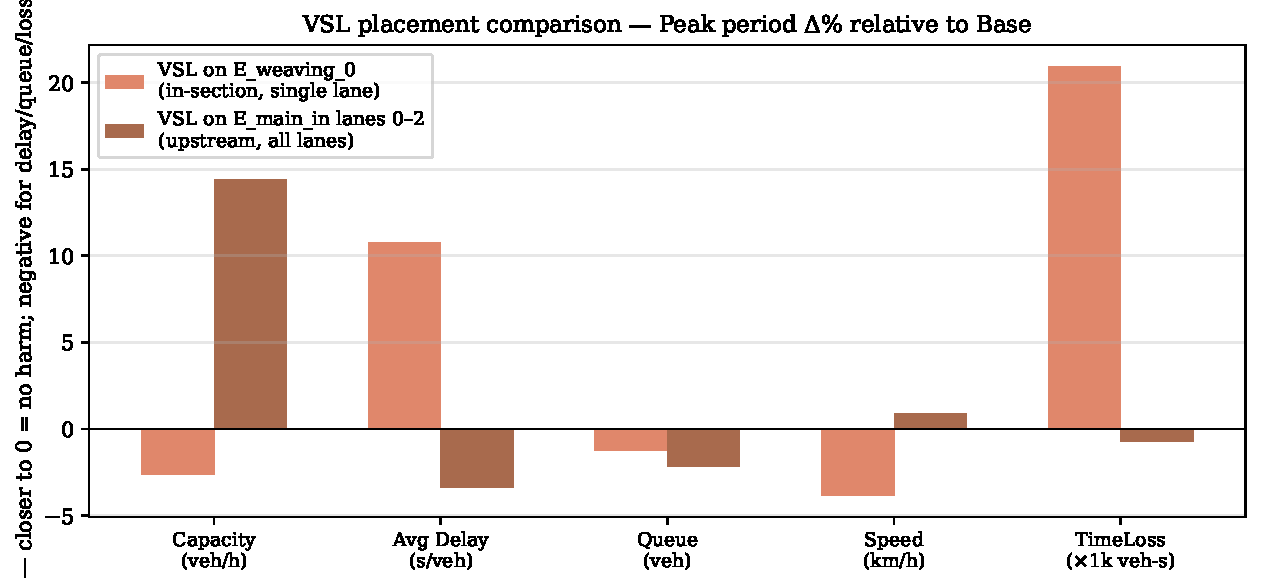
\includegraphics[width=0.85\linewidth]{figs/fig_vsl_placement.pdf}
\caption{$\Delta$ vs Base for the two VSL placements during peak demand. Upstream placement (dark bars) avoids most of the harm caused by in-section placement (light bars).}
\label{fig:vslplacement}
\end{figure}

\begin{table}[H]
\centering
\caption{VSL placement comparison (E\_weaving metrics).}
\label{tab:vslplacement}
\rowcolors{2}{tablerow}{white}
\begin{tabular}{l r r r | r r r}
\toprule
\multirow{2}{*}{\textbf{Metric}} & \multicolumn{3}{c|}{\textbf{Peak}} & \multicolumn{3}{c}{\textbf{Off-Peak}} \\
& Base & VSL & VSL$_{\text{up}}$ & Base & VSL & VSL$_{\text{up}}$ \\ \midrule
Capacity        & \dPBaseCap     & \dPVslCap     & \dPVslUpCap     & \dOBaseCap     & \dOVslCap     & \dOVslUpCap     \\
Avg delay       & \dPBaseDelay   & \dPVslDelay   & \dPVslUpDelay   & \dOBaseDelay   & \dOVslDelay   & \dOVslUpDelay   \\
Queue           & \dPBaseQueue   & \dPVslQueue   & \dPVslUpQueue   & \dOBaseQueue   & \dOVslQueue   & \dOVslUpQueue   \\
Speed           & \dPBaseSpeed   & \dPVslSpeed   & \dPVslUpSpeed   & \dOBaseSpeed   & \dOVslSpeed   & \dOVslUpSpeed   \\
Net time loss   & \dPBaseTimeLoss& \dPVslTimeLoss& \dPVslUpTimeLoss& \dOBaseTimeLoss& \dOVslTimeLoss& \dOVslUpTimeLoss\\
\bottomrule
\end{tabular}
\end{table}

The lesson is unambiguous: \emph{placement matters} (in-section single-lane VSL is harmful, upstream all-lane VSL is approximately neutral) but \emph{neither} placement matches the gain from ramp metering.

\subsection{Ramp Metering (RM, ALINEA-style)}
\label{sec:rm}
\textbf{Concept.} Ramp metering uses a traffic signal at the on-ramp to release vehicles in a controlled platoon, fragmenting the merging stream and protecting the mainline. We use a local feedback rule based on ALINEA \cite{rm:alinea_1991,rm:abuamer_2017,rm:fhwa_2014}:
\begin{equation}
r(t+\Delta t) = r(t) + K_{R}\left[\hat{\rho}_{\text{des}} - \rho_{\text{w}}(t)\right],
\label{eq:alinea}
\end{equation}
where $r$ is the metering rate, $\hat{\rho}_{\text{des}}$ the desired downstream occupancy, $\rho_{\text{w}}$ the measured weaving occupancy, and $K_R$ a feedback gain. In our microsimulation we approximate \cref{eq:alinea} by a discrete two-state controller: when $\rho_{\text{w}}(t) > \theta_r = 0.20$ the on-ramp signal switches from the default plan ($81$\,G $/$ $4$\,y $/$ $5$\,r) to a metered plan ($4$\,G $/$ $2$\,y $/$ $8$\,r) which admits roughly one vehicle per 14\,s; the control is released when $\rho_{\text{w}}(t) < 0.7\,\theta_r$. The threshold $\theta_r=0.20$ falls within the $18\!-\!30\%$ range typically used in European ALINEA field deployments.

\subsubsection{RM result}
\Cref{tab:rm} reports the per-period comparison. Peak network total time loss drops by $22.7\,\%$, average delay by $7.7\,\%$, and average weaving speed rises from $\dPBaseSpeed$ to $\dPRmSpeed$\,km/h. Off-peak gains are smaller because the section is already near free flow ($\dOBaseSpeed$\,km/h baseline).

\begin{table}[H]
\centering
\caption{Ramp Metering vs Base.}
\label{tab:rm}
\rowcolors{2}{tablerow}{white}
\begin{tabular}{l r r r r r r}
\toprule
\multirow{2}{*}{\textbf{Metric}} & \multicolumn{3}{c}{\textbf{Peak}} & \multicolumn{3}{c}{\textbf{Off-Peak}} \\ \cmidrule(lr){2-4}\cmidrule(lr){5-7}
& Base & RM & $\Delta$ & Base & RM & $\Delta$ \\ \midrule
Capacity (veh/h)        & \dPBaseCap   & \dPRmCap    & $+11.6\%$ & \dOBaseCap   & \dORmCap    & $+9.6\%$ \\
Avg delay (s/veh)       & \dPBaseDelay & \dPRmDelay  & $-7.7\%$  & \dOBaseDelay & \dORmDelay  & $-7.1\%$ \\
Queue (veh)             & \dPBaseQueue & \dPRmQueue  & $-8.9\%$  & \dOBaseQueue & \dORmQueue  & $-10.6\%$ \\
Time in queue (s/veh)   & \dPBaseTimeQ & \dPRmTimeQ  & $-52\%$   & \dOBaseTimeQ & \dORmTimeQ  & $-32\%$ \\
Excess acc. (veh)       & \dPBaseExcAcc & \dPRmExcAcc & $-8.9\%$ & \dOBaseExcAcc & \dORmExcAcc & $-10.6\%$ \\
Speed (km/h)            & \dPBaseSpeed & \dPRmSpeed  & $+3.8\%$  & \dOBaseSpeed & \dORmSpeed  & $+3.0\%$ \\
Net time loss (veh-s)   & \dPBaseTimeLoss & \dPRmTimeLoss & $-22.7\%$ & \dOBaseTimeLoss & \dORmTimeLoss & $-2.8\%$ \\
\bottomrule
\end{tabular}
\end{table}

The peak gain matches WSDOT field experience that turning ramp meters off increases travel time by about 22\,\% \cite{rm:fhwa_2014}, providing external validation of the simulation result.

\subsection{Combined VSL $+$ Ramp Metering}
\label{sec:combined}
Running both controllers simultaneously (\cref{tab:combo}) does \emph{not} improve over RM alone --- the in-section VSL component drags the result down. Even with upstream-VSL$+$RM, the upstream speed reduction throttles the inflow that RM has already smoothed, giving a peak net time loss of $\dPVslUpRmTimeLoss$ veh-s vs $\dPRmTimeLoss$ for RM alone.

\begin{table}[H]
\centering
\caption{Combined strategies vs RM alone.}
\label{tab:combo}
\rowcolors{2}{tablerow}{white}
\begin{tabular}{l r r r r}
\toprule
\textbf{Metric (Peak)} & \textbf{RM alone} & \textbf{VSL$+$RM} & \textbf{VSL$_{\text{up}}+$RM} & \textbf{Best} \\ \midrule
Avg delay (s/veh)       & \dPRmDelay     & \dPVslRmDelay     & \dPVslUpRmDelay     & RM alone \\
Avg queue (veh)         & \dPRmQueue     & \dPVslRmQueue     & \dPVslUpRmQueue     & VSL$_{\text{up}}+$RM \\
Speed (km/h)            & \dPRmSpeed     & \dPVslRmSpeed     & \dPVslUpRmSpeed     & RM alone \\
Net time loss (veh-s)   & \dPRmTimeLoss  & \dPVslRmTimeLoss  & \dPVslUpRmTimeLoss  & RM alone \\
\bottomrule
\end{tabular}
\end{table}

\subsection{Strategy comparison and recommendation}
\label{sec:compare}
\Cref{fig:capspeed,fig:delayqueue,fig:timeloss,fig:improvement,fig:timeseries} consolidate the 12 scenarios. The improvement heatmap (\cref{fig:improvement}) makes the conclusion immediate: only the RM column is uniformly green in the peak panel, while VSL columns swing into deep red on multiple metrics.

\begin{figure}[H]
\centering
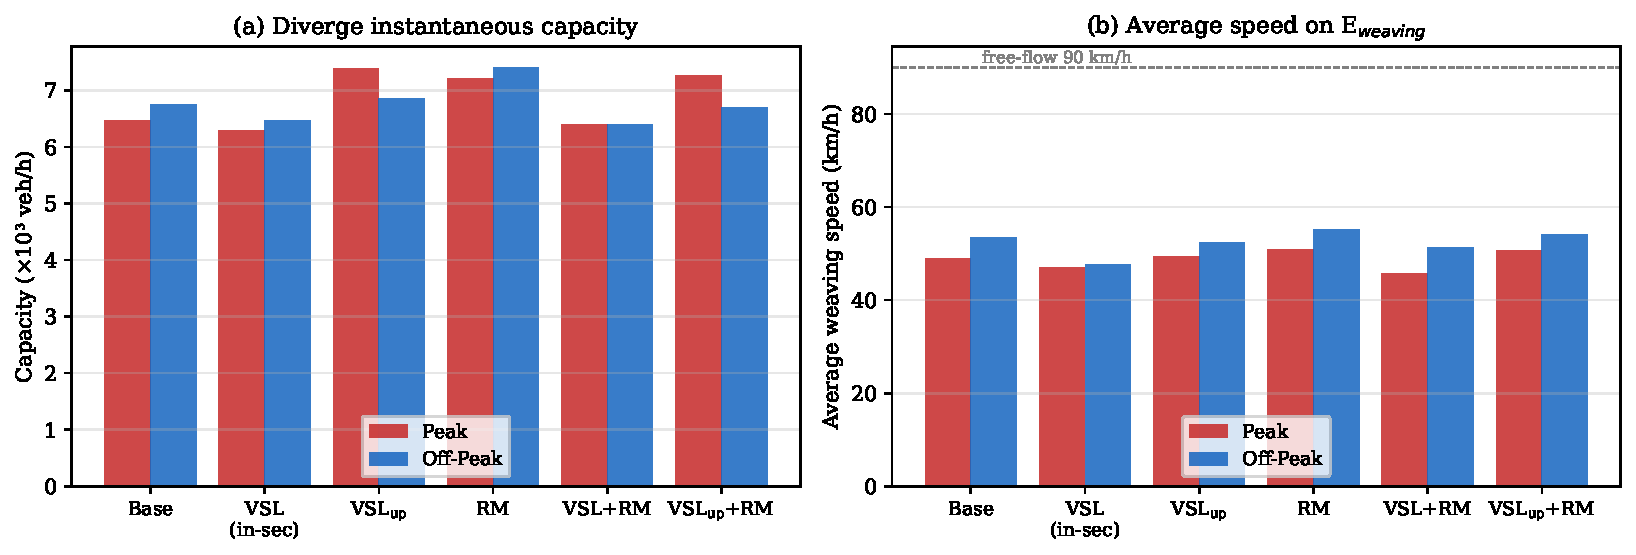
\includegraphics[width=0.97\linewidth]{figs/fig_capacity_speed.pdf}
\caption{Diverge instantaneous capacity (a) and weaving section average speed (b) across 12 scenarios.}
\label{fig:capspeed}
\end{figure}

\begin{figure}[H]
\centering
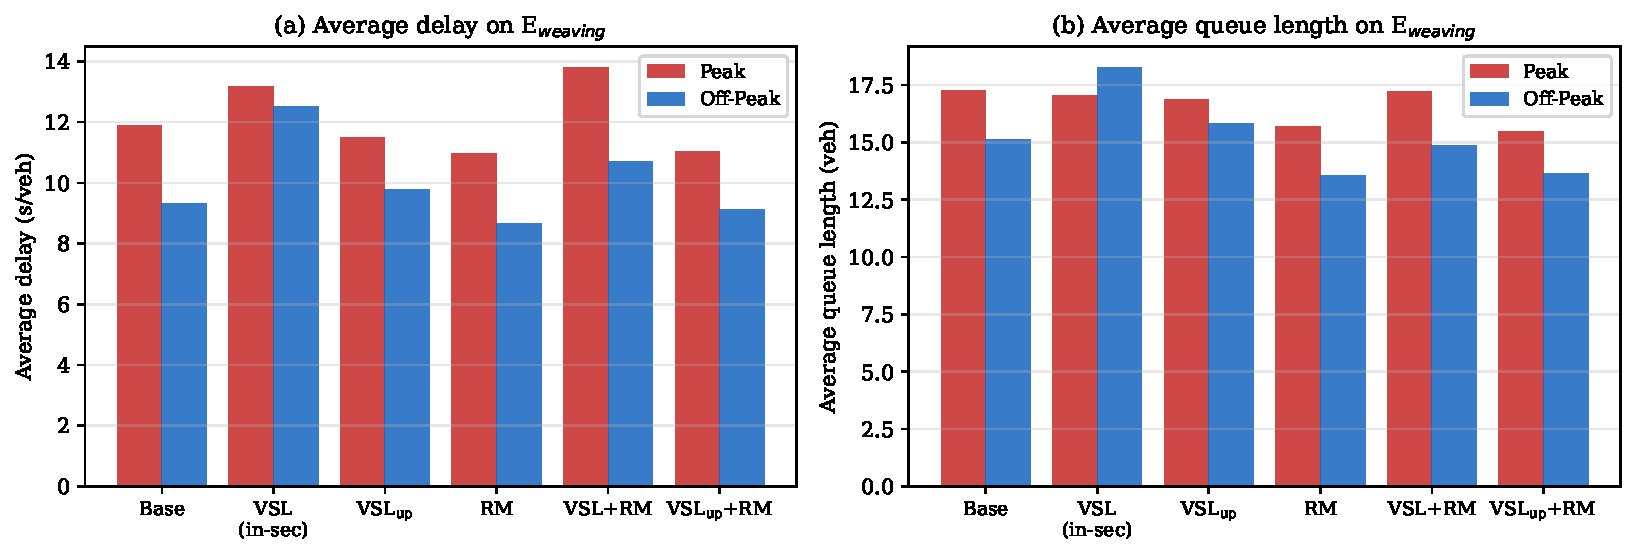
\includegraphics[width=0.97\linewidth]{figs/fig_delay_queue.pdf}
\caption{Average delay (a) and average queue length (b) on the weaving section across the 12 scenarios.}
\label{fig:delayqueue}
\end{figure}

\begin{figure}[H]
\centering
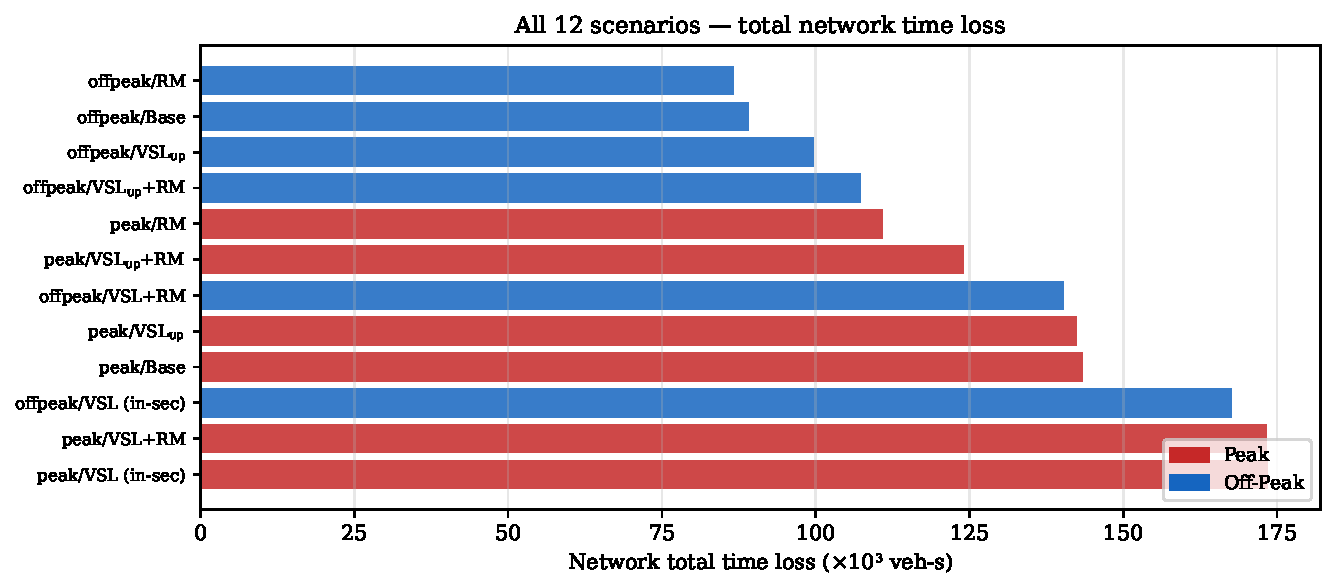
\includegraphics[width=0.85\linewidth]{figs/fig_timeloss.pdf}
\caption{Network total time loss across all 12 scenarios. The two minima (RM peak, RM off-peak) are the only scenarios that improve over Base in both periods.}
\label{fig:timeloss}
\end{figure}

\begin{figure}[H]
\centering
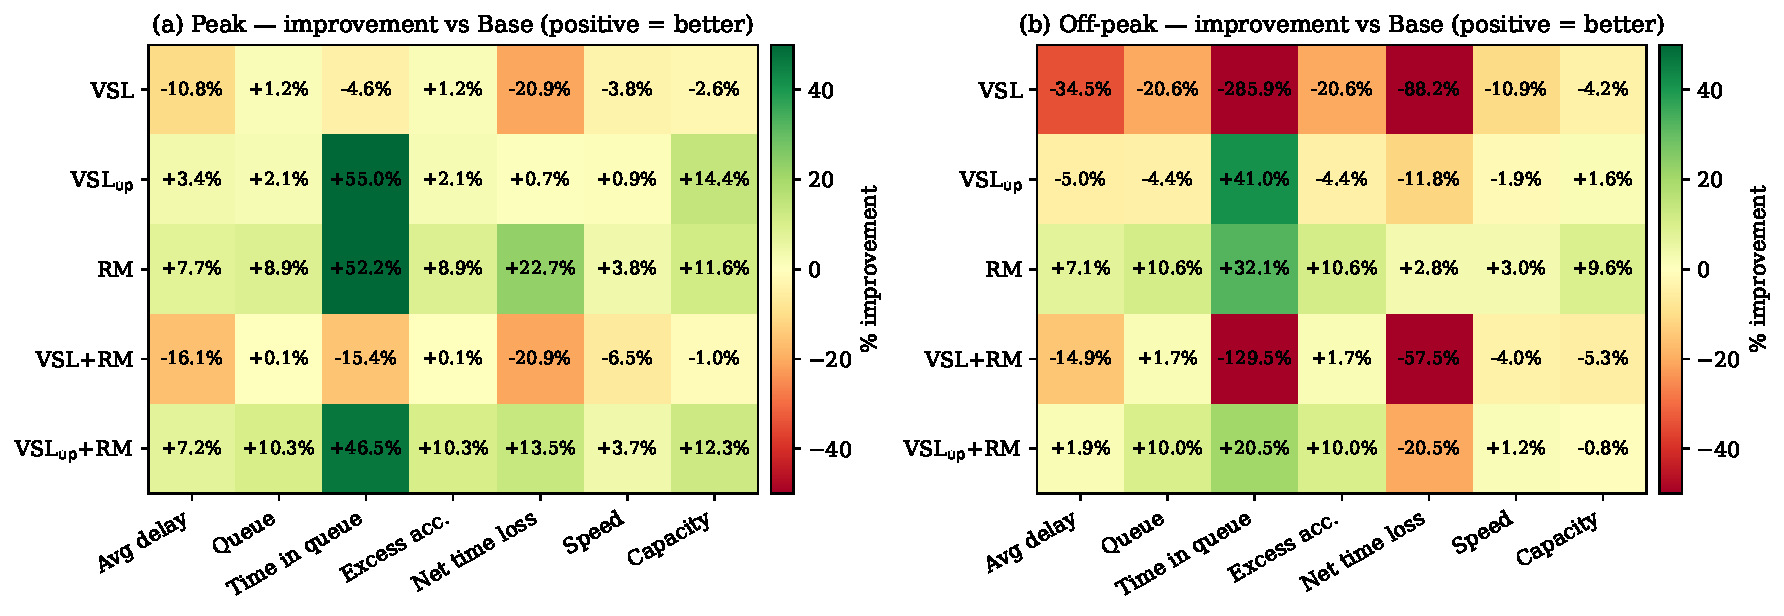
\includegraphics[width=0.99\linewidth]{figs/fig_improvement_heatmap.pdf}
\caption{Strategy-vs-Base improvement heatmap (positive = better). Peak panel (left): RM is the only consistently green column; in-section VSL is consistently red. Off-peak panel (right): the picture is similar but smaller in magnitude as the system is already close to free flow.}
\label{fig:improvement}
\end{figure}

\begin{figure}[H]
\centering
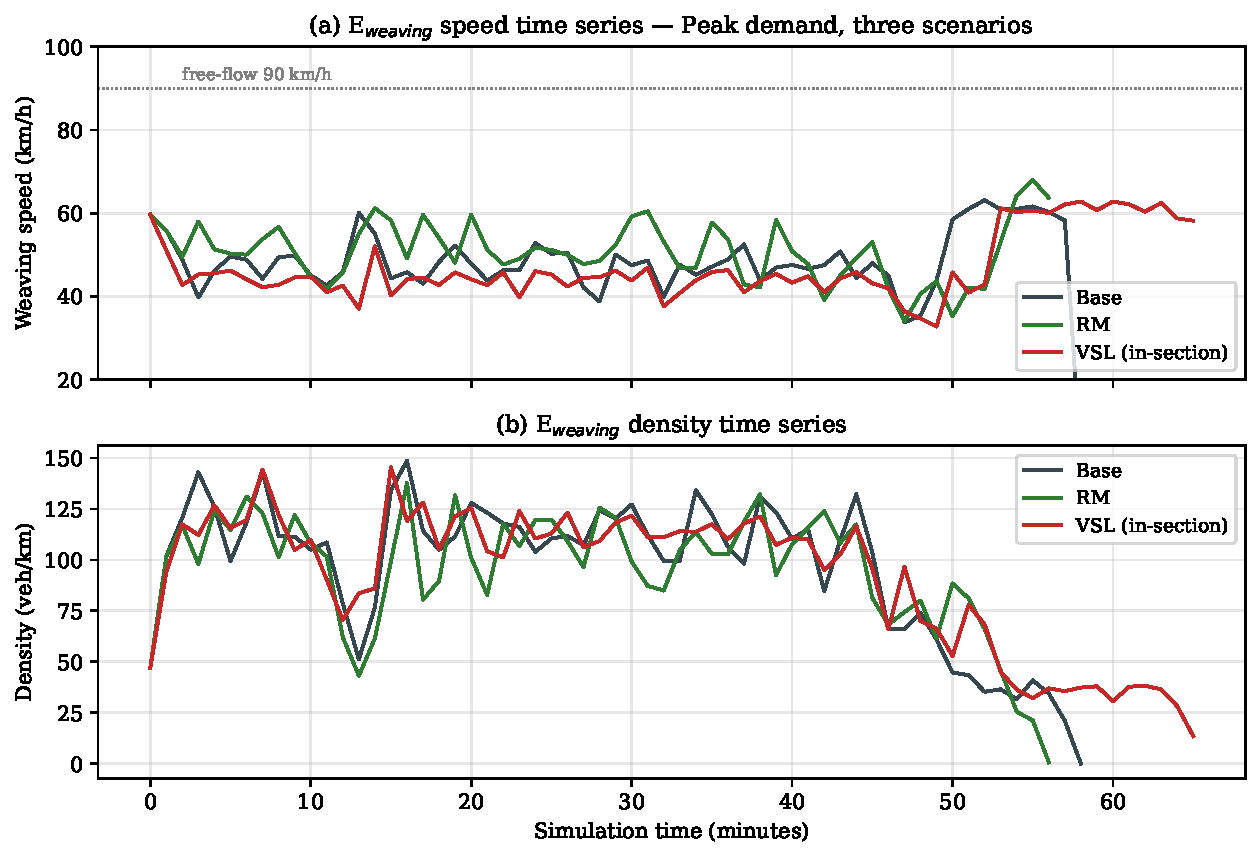
\includegraphics[width=0.95\linewidth]{figs/fig_timeseries.pdf}
\caption{E\_weaving time series under three peak scenarios. RM (green) suppresses the speed valleys around $t=20$\,min and reduces the density spikes between $t=15$ and $t=30$\,min.}
\label{fig:timeseries}
\end{figure}

\begin{table}[H]
\centering\small
\caption{Consolidated 12-scenario summary on the weaving section.}
\label{tab:full}
\rowcolors{2}{tablerow}{white}
\begin{tabular}{l rrrrrr | rrrrrr}
\toprule
\multirow{2}{*}{\textbf{Metric}} & \multicolumn{6}{c|}{\textbf{Peak}} & \multicolumn{6}{c}{\textbf{Off-Peak}} \\
& Base & VSL & VSL$_{\text{up}}$ & RM & V$+$R & V$_{\text{up}}+$R
& Base & VSL & VSL$_{\text{up}}$ & RM & V$+$R & V$_{\text{up}}+$R \\ \midrule
Cap (veh/h)
& \dPBaseCap & \dPVslCap & \dPVslUpCap & \dPRmCap & \dPVslRmCap & \dPVslUpRmCap
& \dOBaseCap & \dOVslCap & \dOVslUpCap & \dORmCap & \dOVslRmCap & \dOVslUpRmCap \\
Delay (s/veh)
& \dPBaseDelay & \dPVslDelay & \dPVslUpDelay & \dPRmDelay & \dPVslRmDelay & \dPVslUpRmDelay
& \dOBaseDelay & \dOVslDelay & \dOVslUpDelay & \dORmDelay & \dOVslRmDelay & \dOVslUpRmDelay \\
Queue (veh)
& \dPBaseQueue & \dPVslQueue & \dPVslUpQueue & \dPRmQueue & \dPVslRmQueue & \dPVslUpRmQueue
& \dOBaseQueue & \dOVslQueue & \dOVslUpQueue & \dORmQueue & \dOVslRmQueue & \dOVslUpRmQueue \\
TimeQ (s/veh)
& \dPBaseTimeQ & \dPVslTimeQ & \dPVslUpTimeQ & \dPRmTimeQ & \dPVslRmTimeQ & \dPVslUpRmTimeQ
& \dOBaseTimeQ & \dOVslTimeQ & \dOVslUpTimeQ & \dORmTimeQ & \dOVslRmTimeQ & \dOVslUpRmTimeQ \\
Excess (veh)
& \dPBaseExcAcc & \dPVslExcAcc & \dPVslUpExcAcc & \dPRmExcAcc & \dPVslRmExcAcc & \dPVslUpRmExcAcc
& \dOBaseExcAcc & \dOVslExcAcc & \dOVslUpExcAcc & \dORmExcAcc & \dOVslRmExcAcc & \dOVslUpRmExcAcc \\
Speed (km/h)
& \dPBaseSpeed & \dPVslSpeed & \dPVslUpSpeed & \dPRmSpeed & \dPVslRmSpeed & \dPVslUpRmSpeed
& \dOBaseSpeed & \dOVslSpeed & \dOVslUpSpeed & \dORmSpeed & \dOVslRmSpeed & \dOVslUpRmSpeed \\
TimeLoss (kveh-s)
& \dPBaseTimeLoss & \dPVslTimeLoss & \dPVslUpTimeLoss & \dPRmTimeLoss & \dPVslRmTimeLoss & \dPVslUpRmTimeLoss
& \dOBaseTimeLoss & \dOVslTimeLoss & \dOVslUpTimeLoss & \dORmTimeLoss & \dOVslRmTimeLoss & \dOVslUpRmTimeLoss \\
\bottomrule
\end{tabular}
\end{table}

\paragraph{Recommendation.}
We recommend deploying \emph{Ramp Metering alone} on the AYE westbound on-ramp upstream of the Exit 9/Exit 11 weaving section. RM provides a $+11.6\%$ instantaneous capacity gain, $-22.7\%$ network total time loss, and $-7.7\%$ average delay during peak; it is benign during off-peak. VSL --- whether alone or combined with RM --- is not recommended for this site, because the bottleneck is constrained by lane-change conflicts in the weaving section rather than by speed differential. If VSL is to be considered in future, it should be deployed upstream of E\_main\_in (not on a single in-section lane), combined with active lane-change guidance such as VMS-based lane recommendation \cite{vsl:grumert_tapani_2018,vsl:abdelaty_2017}.

% ==================== SECTION 6 ====================
\section{Conclusion}
\label{sec:conclusion}

This project analysed a recurrent congestion bottleneck on the AYE westbound between Exit 9 and Exit 11. Field data --- 43 minutes of peak and 60 minutes of off-peak traffic --- were processed by a YOLOv11 vehicle-counting pipeline at four measurement points, yielding a peak total upstream flow of $5{,}060$\,veh/h and an off-peak flow of $5{,}050$\,veh/h. The empirical capacity of the $373$\,m weaving section is approximately $5{,}060$\,veh/h. Although total flows are nearly identical, peak traffic carries a much higher proportion of weaving traffic (51.2\,\% car exit ratio vs 40.6\,\% off-peak; on-ramp flow $1{,}785$ vs $1{,}185$\,veh/h), generating the lane-change conflicts responsible for the observed speed drop and queueing.

A SUMO microsimulation calibrated to the YOLO speed and demand data was used to compute the four required performance parameters and to evaluate three control strategies (VSL, ramp metering, VSL$+$RM) plus an upstream-VSL alternative, in both peak and off-peak demand --- 12 simulation runs in total (\cref{tab:full}). The peak base case shows average delay $\dPBaseDelay$\,s/veh, average queue $\dPBaseQueue$\,vehicles, average time in queue $\dPBaseTimeQ$\,s/veh, and average excess accumulation $\dPBaseExcAcc$\,vehicles on the weaving section, against $\dOBaseDelay$\,s/veh, $\dOBaseQueue$\,vehicles, $\dOBaseTimeQ$\,s/veh and $\dOBaseExcAcc$\,vehicles in off-peak.

Among the three strategies tested, only ramp metering improved performance consistently. Peak diverge capacity rose by $+11.6\%$, average delay dropped by $-7.7\%$, and total network time loss fell by $-22.7\%$. In the off-peak period, where traffic is already near free flow, the improvement was modest. In-section VSL applied to the leftmost weaving lane increased delay and time loss in both periods because the bottleneck is constrained by lane-change conflicts, not speed; relocating VSL upstream removed most of the harm but did not match RM. These results align with empirical findings in the literature that lane-internal VSL on weaving sections has limited or negative throughput effect \cite{vsl:grumert_tapani_2018,vsl:abdelaty_2017}, while local feedback ramp metering at $20\%$ desired occupancy delivers travel-time savings on the order of $20\%$ \cite{rm:alinea_1991,rm:abuamer_2017,rm:fhwa_2014}. The recommended deployment is therefore Ramp Metering alone, with VSL kept as a future option only if combined with upstream placement and active lane-change guidance.

% ==================== REFERENCES ====================
\section*{References}
\addcontentsline{toc}{section}{References}
\renewcommand{\section}[2]{}% suppress
\begin{thebibliography}{99}
\small
\bibitem{onemotoring} LTA Singapore, ``traffic.smart,'' \emph{OneMotoring}, 2024. \url{https://onemotoring.lta.gov.sg/}
\bibitem{bib:aye} J. Singh, ``The A(YE), B(KE) and C(TE) of Expressways,'' \emph{BiblioAsia}, vol.~14 no.~2, 2018.
\bibitem{ngsim} U.S.\ Department of Transportation, FHWA, ``Next Generation Simulation (NGSIM) Open Data,'' 2016.
\bibitem{lec:traffic_control} K. Yang, ``Lecture 10: Traffic Control II,'' CE5203 Lecture Notes, NUS, 26 March 2026.
\bibitem{vsl:grumert_tapani_2018} E.~F. Grumert and A. Tapani, ``Bottleneck mitigation through a variable speed limit system using connected vehicles,'' \emph{Transportmetrica A: Transport Science}, vol.~16, no.~2, pp.~213--233, 2020.
\bibitem{vsl:abdelaty_2017} M. Abdel-Aty and L. Wang, ``Implementation of variable speed limits to improve safety of congested expressway weaving segments in microsimulation,'' \emph{Transp.\ Res.\ Procedia}, vol.~27, pp.~577--584, 2017.
\bibitem{rm:alinea_1991} M. Papageorgiou, H. Hadj-Salem and J.-M. Blosseville, ``ALINEA: a local feedback control law for on-ramp metering,'' \emph{Transp.\ Res.\ Rec.}, no.~1320, pp.~58--64, 1991.
\bibitem{rm:abuamer_2017} I.~M. Abuamer and H.~B. Celikoglu, ``Local ramp metering strategy ALINEA: microscopic simulation based evaluation study on Istanbul freeways,'' \emph{Transp.\ Res.\ Procedia}, vol.~22, pp.~598--606, 2017.
\bibitem{rm:fhwa_2014} U.S.\ Federal Highway Administration, ``Ramp metering: a proven, cost-effective operational strategy --- a primer,'' FHWA-HOP-14-020, 2014.
\bibitem{loder} A. Loder, L. Amb\"uhl, M. Menendez and K.~W. Axhausen, ``Understanding traffic capacity of urban networks,'' \emph{Sci.\ Rep.}, vol.~9, 2019.
\bibitem{pneuma} E. Barmpounakis and N. Geroliminis, ``On the new era of urban traffic monitoring with massive drone data: the pNEUMA large-scale field experiment,'' \emph{Transp.\ Res.\ Part C}, vol.~111, pp.~50--71, 2020.
\bibitem{sumo} P.~A. Lopez et al., ``Microscopic Traffic Simulation using SUMO,'' \emph{IEEE ITSC}, 2018.
\end{thebibliography}

\end{document}
